\documentclass[11pt]{article}

\usepackage[a4paper,margin=2.5cm]{geometry}
\usepackage[T1]{fontenc}
\usepackage{lmodern}
\usepackage{amsmath,amssymb,amsthm,mathtools}
\usepackage{graphicx}
\usepackage{booktabs}
\usepackage{caption}
\usepackage{enumitem}
\usepackage{xcolor}
\usepackage[colorlinks=true,linkcolor=blue!50!black,citecolor=blue!50!black,urlcolor=blue!50!black]{hyperref}

\captionsetup{font=small,labelfont=bf,labelsep=period}
\setlength{\parskip}{2pt}

\newtheorem{theorem}{Theorem}[section]
\newtheorem{lemma}[theorem]{Lemma}
\newtheorem{proposition}[theorem]{Proposition}
\newtheorem{corollary}[theorem]{Corollary}
\theoremstyle{definition}
\newtheorem{definition}[theorem]{Definition}
\newtheorem{remark}[theorem]{Remark}
\newtheorem{example}[theorem]{Example}

\newcommand{\Z}{\mathbb{Z}}
\newcommand{\Q}{\mathbb{Q}}
\newcommand{\E}{\mathcal{E}}
\newcommand{\Hom}{\operatorname{Hom}}
\newcommand{\Gal}{\operatorname{Gal}}
\newcommand{\leg}[2]{\bigl(\tfrac{#1}{#2}\bigr)}
\renewcommand{\phi}{\varphi}
\renewcommand{\epsilon}{\varepsilon}

\hypersetup{
  pdftitle={On the ratio of surjective group homomorphisms to ring homomorphisms between cyclic rings},
  pdfauthor={Priyabrata Mandal, Deep Bhattacharjee}}

\begin{document}

\noindent{\small\itshape Research article}

\vspace{6mm}
\begin{center}
{\Large\bfseries On the ratio of surjective group homomorphisms\\[2pt] to ring homomorphisms between cyclic rings}

\vspace{5mm}
{\large Priyabrata Mandal$^{1,*}$ and Deep Bhattacharjee$^{2}$}

\vspace{3mm}
{\small
$^{1}$ Department of Mathematics, Bioinformatics and Computer Applications, Maulana Azad National Institute of Technology Bhopal, Bhopal 462003, India; ORCID: \href{https://orcid.org/0000-0001-6472-6239}{0000-0001-6472-6239}\\
$^{2}$ Formerly, Electro-Gravitational Space Propulsion Laboratory (EGSPL), Bhubaneswar, Odisha 751030, India; ORCID: \href{https://orcid.org/0000-0003-0466-750X}{0000-0003-0466-750X}\\[2pt]
$^{*}$ \textbf{Correspondence:} Email: \href{mailto:priyabrata@manit.ac.in}{priyabrata@manit.ac.in}; \href{mailto:itsdeep@live.com}{itsdeep@live.com} (D.B.)}
\end{center}

\vspace{4mm}
\noindent\textbf{Abstract:}
For $n\mid m$ there are $\phi(n)$ surjective group homomorphisms $\Z_m\to\Z_n$ and $2^{\omega(n)}$ ring homomorphisms. We show that their ratio $\rho(n)$ is $2^{\epsilon(n)}$ times the number of squares in $(\Z/n\Z)^\times$, where $\epsilon(n)\in\{-1,0,1\}$ is fixed by the power of $2$ dividing $n$, and that for odd $n$ the ring homomorphisms correspond to the subfields of degree at most $2$ of $\Q(\zeta_n)$. We give two-term asymptotic formulas, with explicit constants, for the number of $n\le x$ with $\rho(n)\notin\Z$ and for $\sum_{n\le x}\rho(n)$, and check them against exact computations up to $2\cdot10^{10}$ and $10^{10}$, respectively.

\vspace{2mm}
\noindent\textbf{Keywords:} homomorphisms of cyclic rings; quadratic residues; Selberg--Delange method

\vspace{1mm}
\noindent\textbf{Mathematics Subject Classification:} 11A15, 11N25, 11N37, 11R18, 13M05

\vspace{4mm}

%% ===================================================================
\section{Introduction}\label{sec:intro}
%% ===================================================================

Let $n\mid m$. Gallian and Van Buskirk~\cite{GVB} showed that there are exactly $2^{\omega(n)}$ ring homomorphisms $\Z_m\to\Z_n$, where $\omega(n)$ is the number of distinct prime factors of $n$, and it is elementary that exactly $\phi(n)$ of the group homomorphisms $\Z_m\to\Z_n$ are surjective. This paper is about the ratio
\begin{equation}\label{eq:rho}
  \rho(n)=\frac{\phi(n)}{2^{\omega(n)}} .
\end{equation}
It is often an integer ($\rho(35)=6$, $\rho(120)=4$) and sometimes not ($\rho(6)=\tfrac12$, $\rho(98)=\tfrac{21}{2}$). We determine $\rho(n)$ exactly as a group-theoretic quantity, describe the integers where it fails to be integral, and give two-term asymptotic formulas for how often this happens and for the mean value of~$\rho$.

Write $U_n=(\Z/n\Z)^\times$ and $U_n^2=\{u^2:u\in U_n\}$, so that $|U_n^2|$ is the number of quadratic residues modulo $n$ that are prime to $n$. For $n=2^s n'$ with $n'$ odd put
\begin{equation}\label{eq:eps}
  \epsilon(n)=\begin{cases} 0, & s=0 \text{ or } s=2,\\ -1, & s=1,\\ 1, & s\ge 3,\end{cases}
\end{equation}
and let
\begin{equation}\label{eq:E}
  \E=\{\,n\equiv 2 \!\!\pmod 4:\ \text{every prime divisor of } n/2 \text{ is } \equiv 3 \!\!\pmod 4\,\},
\end{equation}
so that $\E=\{2,6,14,18,22,38,42,46,54,\dots\}$.

\begin{theorem}\label{thm:main}
For every $n\ge1$,
\[
  \rho(n)=2^{\epsilon(n)}\,|U_n^2| .
\]
Moreover, $\rho(n)$ is an integer if and only if $n\notin\E$, and $\rho(n)=|U_n^2|$ whenever $n\not\equiv 2\pmod 4$ and $8\nmid n$.
\end{theorem}

For odd $n$ the identity $|U_n^2|=\phi(n)/2^{\omega(n)}$ is classical, and Theorem~\ref{thm:main} is a short consequence of the structure of $U_n$. We record it because it gives the exact form of $\rho(n)$ for every $n$, and the factor $2^{\epsilon(n)}$ is precisely what produces the set~$\E$. Our second result explains the count $2^{\omega(n)}$ on the field side. Let $\zeta_n=e^{2\pi i/n}$ and, for an odd prime $p$, let $p^*=(-1)^{(p-1)/2}p$.

\begin{theorem}\label{thm:galois}
Let $n$ be odd and $n\mid m$. For a ring homomorphism $f\colon\Z_m\to\Z_n$ let $S(f)$ be the set of primes $p\mid n$ with $f(1)\equiv1\pmod p$, and put $d_f=\prod_{p\in S(f)}p^*$. Then $f\mapsto\Q(\sqrt{d_f})$ is a bijection from the set of ring homomorphisms $\Z_m\to\Z_n$ onto the set of subfields $K\subseteq\Q(\zeta_n)$ with $[K:\Q]\le2$. Moreover $\rho(n)=[\Q(\zeta_n):M_n]$, where $M_n$ is the compositum of these fields.
\end{theorem}

The bijection comes from an isomorphism between the Boolean group of idempotents of $\Z/n\Z$ and the group of quadratic characters of $U_n$ (Proposition~\ref{prop:iso}). Figure~\ref{fig:cube} shows it for $n=105$. For even $n$ the two groups have orders $2^{\omega(n)}$ and $2^{\omega(n)+\epsilon(n)}$, which is another way of reading Theorem~\ref{thm:main}.

The remaining results are analytic. Let $\E(x)=\#\{n\le x:n\in\E\}$, let $\chi_{-4}$ be the non-principal character modulo $4$, and let $\gamma$ be Euler's constant.

\begin{theorem}\label{thm:exc}
As $x\to\infty$,
\[
  \E(x)=\frac{Cx}{\sqrt{\log x}}\Bigl(1+\frac{\kappa}{\log x}+O\Bigl(\frac{1}{(\log x)^2}\Bigr)\Bigr),
\]
where
\begin{align*}
  C&=\frac{1}{\pi\sqrt2}\prod_{p\equiv3\,(4)}\Bigl(1-\frac1{p^2}\Bigr)^{-1/2}=0.24325\,99441\,92945\ldots,\\
  \kappa&=\frac12-\frac{\gamma}{4}+\frac{\log2}{4}+\frac12\sum_{p\equiv3\,(4)}\frac{\log p}{p^2-1}+\frac14\,\frac{L'(1,\chi_{-4})}{L(1,\chi_{-4})}=0.70475\,34517\,05947\ldots .
\end{align*}
\end{theorem}

\begin{theorem}\label{thm:mean}
As $x\to\infty$,
\[
  \sum_{n\le x}\rho(n)=\frac{C_2x^2}{\sqrt{\log x}}\Bigl(1+\frac{\kappa_2}{\log x}+O\Bigl(\frac{1}{(\log x)^2}\Bigr)\Bigr),
\]
where
\begin{align*}
  C_2&=\frac{1}{2\sqrt\pi}\prod_{p}\Bigl(1+\frac1{2p}\Bigr)\Bigl(1-\frac1p\Bigr)^{1/2}=0.22909\,07914\,88938\ldots,\\
  \kappa_2&=\frac14-\frac{\gamma}{4}-\frac14\sum_{p}\frac{\log p}{(2p+1)(p-1)}=0.02482\,64240\,33851\ldots .
\end{align*}
\end{theorem}

Both main terms fit into known results. The set $\E$ is twice the set of odd integers composed of primes $\equiv3\pmod4$. Counting problems of this kind go back to Landau's work on sums of two squares, and such counting functions have asymptotic expansions in powers of $1/\log x$ (see Moree~\cite{Moree}); the leading constant $2C$ for our set appears explicitly in the work of Jones and Zvonkin~\cite{JZ}. Finch and Sebah~\cite{FS} obtained the leading term of $\sum_{n\le x}|U_n^2|$; since $\rho(n)$ and $|U_n^2|$ differ only by the factor $2^{\epsilon(n)}$, their constant is $\tfrac{43}{40}C_2$. What we add is closed forms for the second-order coefficients $\kappa$ and $\kappa_2$, self-contained proofs of both two-term expansions by the Selberg--Delange method~\cite[Theorem~II.5.2]{Ten}, and a comparison with exact computations of $\E(x)$ up to $x=2\cdot10^{10}$ and of $\sum_{n\le x}\rho(n)$ up to $x=10^{10}$.

Section~\ref{sec:prelim} collects the counting lemmas. Theorem~\ref{thm:main} is proved in Section~\ref{sec:exact}, Theorem~\ref{thm:galois} in Section~\ref{sec:galois}, and Theorems~\ref{thm:exc} and~\ref{thm:mean} in Section~\ref{sec:analytic}, which ends with the numerical comparison.

%% ===================================================================
\section{Preliminaries}\label{sec:prelim}
%% ===================================================================

Ring homomorphisms are not required to send $1$ to $1$; this is the convention of~\cite{GVB}.\footnote{If one insists on $f(1)=1$, there is exactly one ring homomorphism $\Z_m\to\Z_n$ when $n\mid m$, and the question studied here disappears.} We write $B_n=\{e\in\Z/n\Z:e^2=e\}$ for the set of idempotents.

\begin{lemma}\label{lem:ring}
Let $n\mid m$. The map $f\mapsto f(1)$ is a bijection from the ring homomorphisms $\Z_m\to\Z_n$ onto $B_n$, and $|B_n|=2^{\omega(n)}$.
\end{lemma}

\begin{proof}
An additive map satisfies $f(k)=kf(1)$, and multiplicativity gives $f(1)=f(1)^2$. Conversely, if $e\in B_n$ then $k\mapsto ke$ is well defined on $\Z_m$ because $n\mid m$, it is additive, and $(ab)e=(ab)e^2=(ae)(be)$. Write $n=\prod_{i=1}^{k}p_i^{r_i}$. By the Chinese remainder theorem $\Z/n\Z\cong\prod_i\Z/p_i^{r_i}\Z$, and each factor is a local ring, whose only idempotents are $0$ and $1$. Hence $|B_n|=2^k$.
\end{proof}

The proof shows more. The map $e\mapsto S(e)=\{p_i: e\equiv1\pmod{p_i}\}$ is a bijection from $B_n$ onto the subsets of $\{p_1,\dots,p_k\}$; note that $e\equiv1\pmod{p_i}$ forces $e\equiv1\pmod{p_i^{r_i}}$, since $e\bmod p_i^{r_i}\in\{0,1\}$. With the Boolean sum $e\oplus e'=e+e'-2ee'$, which reduces to addition modulo $2$ in each component, $B_n$ is an elementary abelian $2$-group and
\begin{equation}\label{eq:symdiff}
  S(e\oplus e')=S(e)\,\triangle\,S(e').
\end{equation}

\begin{lemma}\label{lem:surj}
Let $n\mid m$. Exactly $\phi(n)$ group homomorphisms $\Z_m\to\Z_n$ are surjective.
\end{lemma}

\begin{proof}
Group homomorphisms are $k\mapsto ka$ with $a\in\Z_n$ (well defined since $n\mid m$), and $k\mapsto ka$ is onto exactly when $\gcd(a,n)=1$.
\end{proof}

\begin{lemma}\label{lem:index}
For every $n\ge1$, $[U_n:U_n^2]=2^{\omega(n)+\epsilon(n)}$.
\end{lemma}

\begin{proof}
For a finite abelian group $A$ the squaring map has kernel $A[2]$, so $[A:A^2]=|A[2]|$, and a cyclic group contributes a factor $2$ to $|A[2]|$ if its order is even and $1$ otherwise. By the Chinese remainder theorem $U_n\cong\prod_{p^r\Vert n}U_{p^r}$. For odd $p$ the group $U_{p^r}$ is cyclic of even order $p^{r-1}(p-1)$; moreover $U_2=1$, $U_4\cong\Z/2$, and $U_{2^s}\cong\Z/2\times\Z/2^{s-2}$ for $s\ge3$ \cite[Chapter~4]{IR}. If $n=2^sn'$ with $n'$ odd, this gives $[U_n:U_n^2]=2^{\omega(n')+t}$ with $t=0,0,1,2$ for $s=0$, $s=1$, $s=2$, $s\ge3$. Since $\omega(n)=\omega(n')+[s\ge1]$, the exponent is $\omega(n)+\epsilon(n)$ in every case.
\end{proof}

%% ===================================================================
\section{The exact value of \texorpdfstring{$\rho(n)$}{rho(n)}}\label{sec:exact}
%% ===================================================================

\begin{proof}[Proof of Theorem~\ref{thm:main}]
By Lemma~\ref{lem:index}, $\phi(n)=|U_n|=|U_n^2|\,[U_n:U_n^2]=|U_n^2|\,2^{\omega(n)+\epsilon(n)}$. Dividing by $2^{\omega(n)}$ gives $\rho(n)=2^{\epsilon(n)}|U_n^2|$.

If $\epsilon(n)\ge0$, then $\rho(n)$ is an integer and $n\notin\E$. Let $\epsilon(n)=-1$, that is $n=2n'$ with $n'$ odd. Then $U_n\cong U_{n'}$, so $\rho(n)=\tfrac12|U_{n'}^2|$ with
\[
  |U_{n'}^2|=\prod_{p^r\Vert n'}\frac{p^{r-1}(p-1)}{2}
\]
by Lemma~\ref{lem:index} applied to each cyclic factor. A factor $p^{r-1}(p-1)/2$ is even exactly when $p\equiv1\pmod4$. So $\rho(n)\in\Z$ if and only if some prime divisor of $n'$ is $\equiv1\pmod4$, which means $n\notin\E$. For $n=2$ the product is empty, so $\rho(2)=\tfrac12$, and indeed $2\in\E$. The last assertion is the case $\epsilon(n)=0$.
\end{proof}

Equivalently, $2^{\omega(n)}\mid\phi(n)$ if and only if $n\notin\E$. Table~\ref{tab:small} shows each case. Note that $\rho(n)$ and $|U_n^2|$ really do differ when $n\equiv2\pmod4$ or $8\mid n$: for $n=26$ the ratio is $3$ while there are $6$ unit squares, and for $n=120$ the ratio is $4$ while there are $2$.

\begin{table}[htbp]
\centering
\caption{The quantities of Theorem~\ref{thm:main} for some small $n$.}
\label{tab:small}
\small
\begin{tabular}{rlrrrrrc}
\toprule
$n$ & factorisation & $\epsilon(n)$ & $\phi(n)$ & $2^{\omega(n)}$ & $|U_n^2|$ & $\rho(n)$ & $n\in\E$\\
\midrule
$2$ & $2$ & $-1$ & $1$ & $2$ & $1$ & $1/2$ & yes \\
$6$ & $2\cdot 3$ & $-1$ & $2$ & $4$ & $1$ & $1/2$ & yes \\
$10$ & $2\cdot 5$ & $-1$ & $4$ & $4$ & $2$ & $1$ & no \\
$12$ & $2^{2}\cdot 3$ & $0$ & $4$ & $4$ & $1$ & $1$ & no \\
$24$ & $2^{3}\cdot 3$ & $1$ & $8$ & $4$ & $1$ & $2$ & no \\
$26$ & $2\cdot 13$ & $-1$ & $12$ & $4$ & $6$ & $3$ & no \\
$35$ & $5\cdot 7$ & $0$ & $24$ & $4$ & $6$ & $6$ & no \\
$45$ & $3^{2}\cdot 5$ & $0$ & $24$ & $4$ & $6$ & $6$ & no \\
$98$ & $2\cdot 7^{2}$ & $-1$ & $42$ & $4$ & $21$ & $21/2$ & yes \\
$105$ & $3\cdot 5\cdot 7$ & $0$ & $48$ & $8$ & $6$ & $6$ & no \\
$120$ & $2^{3}\cdot 3\cdot 5$ & $1$ & $32$ & $8$ & $2$ & $4$ & no \\
\bottomrule
\end{tabular}
\end{table}

%% ===================================================================
\section{The cyclotomic picture}\label{sec:galois}
%% ===================================================================

Let $G_n=\Gal(\Q(\zeta_n)/\Q)$. The map $u\mapsto\sigma_u$, $\sigma_u(\zeta_n)=\zeta_n^u$, is an isomorphism $U_n\to G_n$ \cite[Chapter~2]{Wash}, and we identify the two groups. Let $X_n=\Hom(U_n,\{\pm1\})$ be the group of characters of order at most $2$. Since $U_n/U_n^2$ is an elementary abelian $2$-group, $|X_n|=[U_n:U_n^2]$, and $\chi\mapsto\ker\chi$ is a bijection from $X_n$ onto the subgroups of index at most $2$ in $U_n$.

\begin{definition}\label{def:Mn}
$M_n$ is the fixed field of $U_n^2$ in $\Q(\zeta_n)$.
\end{definition}

\begin{proposition}\label{prop:Mn}
Let $n\ge1$ and put $w=\omega(n)+\epsilon(n)$.
\begin{enumerate}[label=\upshape(\roman*)]
\item A subfield $K\subseteq\Q(\zeta_n)$ satisfies $K\subseteq M_n$ if and only if $\Gal(K/\Q)$ has exponent at most $2$. In particular $M_n$ is the compositum of all quadratic subfields of $\Q(\zeta_n)$.
\item $[M_n:\Q]=2^{w}$, $[\Q(\zeta_n):M_n]=|U_n^2|$, and $\Q(\zeta_n)$ has exactly $2^{w}-1$ quadratic subfields.
\item $M_n=\Q\bigl(\{\sqrt{p^*}:p\mid n,\ p \text{ odd}\}\cup\{\sqrt{-1}:4\mid n\}\cup\{\sqrt2:8\mid n\}\bigr)$.
\end{enumerate}
\end{proposition}

\begin{proof}
(i) Every subfield $K$ is Galois over $\Q$, and $\Gal(K/\Q)\cong U_n/H$ where $H$ fixes $K$. This quotient has exponent at most $2$ if and only if $H\supseteq U_n^2$, that is $K\subseteq M_n$. In the elementary abelian $2$-group $U_n/U_n^2$ the trivial subgroup is the intersection of the subgroups of index $2$, so $U_n^2$ is the intersection of the subgroups of index $2$ of $U_n$ that contain it. By the Galois correspondence, $M_n$ is the compositum of the quadratic subfields of $\Q(\zeta_n)$.

(ii) The degrees follow from Lemma~\ref{lem:index} and the Galois correspondence. The quadratic subfields correspond to subgroups of index $2$ containing $U_n^2$, that is to the $2^w-1$ non-trivial elements of $X_n$.

(iii) Let $a_1,\dots,a_t$ be the listed radicands. Each $\sqrt{a_j}$ lies in $\Q(\zeta_n)$: for odd $p\mid n$ the Gauss sum $g_p=\sum_{a=1}^{p-1}\leg{a}{p}\zeta_p^{a}$ satisfies $g_p^2=p^*$ \cite[Proposition~6.3.2]{IR}; $\sqrt{-1}=\zeta_4$; and $\sqrt2=\zeta_8+\zeta_8^{-1}$. Counting the radicands gives $t=\omega(n')+[4\mid n]+[8\mid n]=w$, where $n'$ is the odd part of $n$. The $2^w-1$ numbers $\prod_{j\in J}a_j$ with $\emptyset\ne J\subseteq\{1,\dots,t\}$ are pairwise distinct modulo $\Q^{\times2}$. Indeed, a quotient of two of them is, up to a square, again a product over a non-empty set of radicands, and such a product is never a square: an odd prime in it occurs to the first power, and without odd primes it is $-1$, $2$ or $-2$. So they define $2^w-1$ distinct quadratic subfields of $\Q(\zeta_n)$, which by (ii) are all of them. By (i) their compositum is $M_n$, and it equals $\Q(\sqrt{a_1},\dots,\sqrt{a_t})$.
\end{proof}

We call $M_n$ the maximal multiquadratic subfield of $\Q(\zeta_n)$.\footnote{For odd $n$ with $k$ distinct prime factors, $[M_n:\Q]=2^k$, so $M_n$ is biquadratic only when $k=2$.} For odd $p$ and $u\in U_n$,
\begin{equation}\label{eq:gauss-action}
  \sigma_u(g_p)=\sum_{a=1}^{p-1}\leg{a}{p}\zeta_p^{ua}=\leg{u}{p}\sum_{a=1}^{p-1}\leg{ua}{p}\zeta_p^{ua}=\leg{u}{p}g_p .
\end{equation}

From now on let $n$ be odd. For $e\in B_n$ define
\[
  \chi_e(u)=\prod_{p\in S(e)}\leg{u}{p}\quad(u\in U_n),\qquad d_e=\prod_{p\in S(e)}p^*,\qquad \gamma_e=\prod_{p\in S(e)}g_p ,
\]
so that $\chi_0=1$, $d_0=1$, $\gamma_0=1$.

\begin{proposition}\label{prop:iso}
Let $n$ be odd. Then $e\mapsto\chi_e$ is a group isomorphism $(B_n,\oplus)\to X_n$, and for every $e\in B_n$ the fixed field of $\ker\chi_e$ is $\Q(\sqrt{d_e})$.
\end{proposition}

\begin{proof}
Each $\chi_e$ is a product of characters of order dividing $2$, so $\chi_e\in X_n$. By~\eqref{eq:symdiff}, $\chi_{e\oplus e'}=\chi_e\chi_{e'}$, because a prime in $S(e)\cap S(e')$ contributes $\leg{u}{p}^2=1$. If $e\ne0$, choose $p\in S(e)$, a quadratic non-residue $v$ modulo $p$, and $u\in U_n$ with $u\equiv v\pmod p$ and $u\equiv1$ modulo every other prime power dividing $n$; then $\chi_e(u)=-1$. Hence the homomorphism is injective. Both groups have order $2^{\omega(n)}$, by Lemma~\ref{lem:ring} and by $|X_n|=[U_n:U_n^2]$ with Lemma~\ref{lem:index}, so it is bijective.

By~\eqref{eq:gauss-action}, $\sigma_u(\gamma_e)=\chi_e(u)\gamma_e$, and $\gamma_e^2=d_e$. Hence $\sigma_u$ fixes $\Q(\gamma_e)=\Q(\sqrt{d_e})$ exactly when $u\in\ker\chi_e$, and the Galois correspondence gives the claim.
\end{proof}

\begin{proof}[Proof of Theorem~\ref{thm:galois}]
Compose three bijections: $f\mapsto f(1)$ from ring homomorphisms onto $B_n$ (Lemma~\ref{lem:ring}); $e\mapsto\ker\chi_e$ from $B_n$ onto the subgroups of index at most $2$ in $U_n$ (Proposition~\ref{prop:iso}); and the Galois correspondence from these subgroups onto the subfields of degree at most $2$. By Proposition~\ref{prop:iso} the composite sends $f$ to $\Q(\sqrt{d_{f(1)}})=\Q(\sqrt{d_f})$. Finally, $\epsilon(n)=0$ for odd $n$, so Theorem~\ref{thm:main} and Proposition~\ref{prop:Mn}(ii) give $\rho(n)=|U_n^2|=[\Q(\zeta_n):M_n]$.
\end{proof}

\begin{figure}[htbp]
\centering
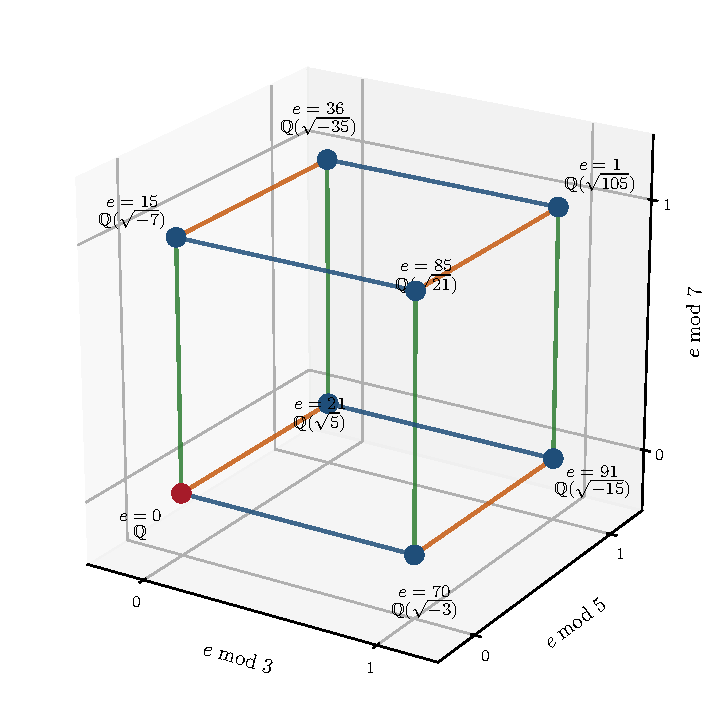
\includegraphics[width=0.62\textwidth]{figures/fig1_cube.pdf}
\caption{Theorem~\ref{thm:galois} for $n=105$. The eight idempotents $e$ of $\Z/105\Z$ sit at the vertices $(e\bmod3,\,e\bmod5,\,e\bmod7)$ of the cube, and each is labelled with the field $\Q(\sqrt{d_e})\subseteq\Q(\zeta_{105})$. Moving along an edge changes one coordinate, which is the Boolean sum with $70$, $21$ or $15$ (blue, orange and green edges), and multiplies $d_e$ by $-3$, $5$ or $-7$ modulo squares. The compositum of the seven quadratic fields is $M_{105}=\Q(\sqrt{-3},\sqrt5,\sqrt{-7})$, and $[\Q(\zeta_{105}):M_{105}]=48/8=6=\rho(105)$.}
\label{fig:cube}
\end{figure}

\begin{remark}\label{rem:even}
For even $n$ the groups $B_n$ and $X_n$ have orders $2^{\omega(n)}$ and $2^{\omega(n)+\epsilon(n)}$. When $4\Vert n$ they are still isomorphic: the $2$-component of $e$ is matched with the character $u\mapsto(-1)^{(u-1)/2}$, whose field is $\Q(\sqrt{-1})$. When $n\equiv2\pmod4$ the $2$-component of $e$ has no character to go to, because $U_2$ is trivial, and when $8\mid n$ there are two independent characters of $U_{2^s}$ and only one idempotent component. This mismatch is the factor $2^{\epsilon(n)}$ in Theorem~\ref{thm:main}.
\end{remark}

Figure~\ref{fig:torus} shows the same structure inside a single unit group. With generators $2$ of $U_5$ and $3$ of $U_7$, the group $U_{35}\cong\Z/4\times\Z/6$ is drawn on a torus. The two characters $\leg{\cdot}{5}$ and $\leg{\cdot}{7}$ split it into four cosets of $U_{35}^2$, and the coset of squares has $6=\rho(35)$ elements.

\begin{figure}[htbp]
\centering
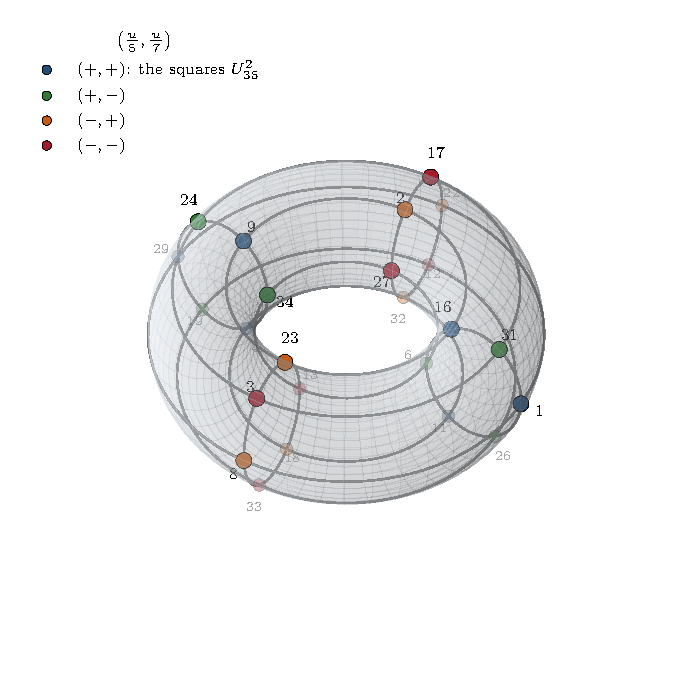
\includegraphics[width=0.72\textwidth]{figures/fig2_torus.pdf}
\caption{The $24$ elements of $U_{35}$ on a torus: $u$ is placed at angle $2\pi k/4$ around the core circle and $2\pi l/6$ around the tube, where $u\equiv2^k\pmod5$ and $u\equiv3^l\pmod7$. The colour records $\bigl(\leg{u}{5},\leg{u}{7}\bigr)$. The six blue points $\{1,4,9,11,16,29\}$ form $U_{35}^2$, the subgroup fixing $M_{35}=\Q(\sqrt5,\sqrt{-7})$. Labels of points on the far side of the torus are drawn faint.}
\label{fig:torus}
\end{figure}

%% ===================================================================
\section{Distribution}\label{sec:analytic}
%% ===================================================================

Write $s=\sigma+i\tau$. We use the Selberg--Delange method in the following form \cite[Theorem~II.5.2]{Ten}, specialised to non-negative coefficients and two terms.

\begin{lemma}\label{lem:SD}
Let $a_n\ge0$ and let $F(s)=\sum_{n\ge1}a_nn^{-s}$ converge for $\sigma>1$. Suppose there are $z>0$, $c_0>0$, $0<\delta\le1$ and $M>0$ such that $G(s)=F(s)\zeta(s)^{-z}$ extends holomorphically to the region $D=\{\sigma\ge1-c_0/(1+\log(1+|\tau|))\}$ and satisfies $|G(s)|\le M(1+|\tau|)^{1-\delta}$ there. Put $Z(s)=((s-1)\zeta(s))^{z}G(s)/s$. Then, for $x\ge3$,
\[
  \sum_{n\le x}a_n=x(\log x)^{z-1}\Bigl(\lambda_0+\frac{\lambda_1}{\log x}+O\Bigl(\frac{1}{(\log x)^2}\Bigr)\Bigr),
  \qquad
  \lambda_0=\frac{Z(1)}{\Gamma(z)},\quad\lambda_1=\frac{Z'(1)}{\Gamma(z-1)} .
\]
\end{lemma}

For $z=\tfrac12$ we have $\Gamma(\tfrac12)=\sqrt\pi$ and $\Gamma(-\tfrac12)=-2\sqrt\pi$. Since $(s-1)\zeta(s)=1+\gamma(s-1)+O((s-1)^2)$,
\begin{equation}\label{eq:Zprime}
  \frac{Z'(1)}{Z(1)}=\frac{\gamma}{2}+\frac{G'(1)}{G(1)}-1,
  \qquad\text{so}\qquad
  \frac{\lambda_1}{\lambda_0}=-\frac12\Bigl(\frac{\gamma}{2}+\frac{G'(1)}{G(1)}-1\Bigr)\quad\Bigl(z=\tfrac12\Bigr).
\end{equation}

\subsection{The exceptional set}

Let $\mathcal A$ be the set of odd $a\ge1$ all of whose prime factors are $\equiv3\pmod4$. By~\eqref{eq:E}, $\E=\{2a:a\in\mathcal A\}$, so $\E(x)=A(x/2)$ with $A(y)=\#\{a\le y:a\in\mathcal A\}$. For $\sigma>1$ put
\[
  P(s)=\sum_{a\in\mathcal A}a^{-s}=\prod_{p\equiv3\,(4)}\bigl(1-p^{-s}\bigr)^{-1},\qquad L(s)=L(s,\chi_{-4}).
\]
Comparing Euler factors at $p=2$, at $p\equiv1\pmod4$ and at $p\equiv3\pmod4$ gives, for $\sigma>1$,
\begin{equation}\label{eq:Psquare}
  P(s)^2=\frac{(1-2^{-s})\,\zeta(s)\,P(2s)}{L(s)} .
\end{equation}
Indeed, at $p\equiv3\pmod4$ the right side has factor $(1-p^{-s})^{-1}(1+p^{-s})(1-p^{-2s})^{-1}=(1-p^{-s})^{-2}$, and at the other primes all factors cancel. Iterating~\eqref{eq:Psquare} at $s=2,4,8,\dots$ gives a rapidly convergent formula,
\begin{equation}\label{eq:P2}
  P(2)=\prod_{j\ge1}\Bigl(\frac{(1-2^{-2^j})\,\zeta(2^j)}{L(2^j)}\Bigr)^{2^{-j}}=1.16807\,55854\,10514\ldots,
\end{equation}
which is how the value of $C$ was computed.\footnote{The first factor involves $L(2)$, which is Catalan's constant. A direct product over the primes $p<10^7$ agrees with~\eqref{eq:P2} to eight decimal places, as the size of the omitted tail predicts.}

\begin{proof}[Proof of Theorem~\ref{thm:exc}]
By~\eqref{eq:Psquare}, $G(s)=P(s)\zeta(s)^{-1/2}$ satisfies, for $\sigma>1$,
\[
  G(s)^2=R(s):=\frac{(1-2^{-s})\,P(2s)}{L(s)} .
\]
The product $P(2s)$ converges absolutely and has no zeros for $\sigma>\tfrac12$, and $1-2^{-s}\ne0$ for $\sigma>0$. Since the modulus is fixed, there is $c>0$ such that $L(s)\ne0$ and $1/L(s)\ll\log(|\tau|+3)$ for $\sigma\ge1-c/\log(|\tau|+3)$ \cite[Chapter~11]{MV}. Choose $c_0>0$ so small that the region $D$ of Lemma~\ref{lem:SD} lies inside this zero-free region and inside $\sigma>\tfrac34$. Then $R$ is holomorphic and zero-free on $D$, and $D$ is simply connected, so $R$ has a holomorphic square root on $D$; we take the one that agrees with $G$ on $\sigma>1$ (two continuous square roots of the same zero-free function on a connected set agree once they agree at one point). On $D$ we have $|R(s)|\ll\log(|\tau|+3)$, so $|G(s)|\ll(1+|\tau|)^{1/2}$ and Lemma~\ref{lem:SD} applies with $z=\delta=\tfrac12$.

Since $L(1)=\pi/4$ and $R(\sigma)>0$ for real $\sigma\ge1$,
\[
  Z(1)=G(1)=\sqrt{R(1)}=\Bigl(\frac{2P(2)}{\pi}\Bigr)^{1/2},\qquad
  \frac{G'(1)}{G(1)}=\frac12\,\frac{R'(1)}{R(1)}=\frac12\Bigl(\log2-2\Sigma_3-\frac{L'(1)}{L(1)}\Bigr),
\]
where $\Sigma_3=\sum_{p\equiv3\,(4)}\log p/(p^2-1)=-P'(2)/P(2)$. Lemma~\ref{lem:SD} gives
\[
  A(y)=\frac{y}{\sqrt{\log y}}\Bigl(\lambda_0+\frac{\lambda_1}{\log y}+O\Bigl(\frac1{(\log y)^2}\Bigr)\Bigr),\qquad
  \lambda_0=\frac{\sqrt{2P(2)}}{\pi},
\]
with $\lambda_1/\lambda_0$ given by~\eqref{eq:Zprime}. Put $y=x/2$. Since $(\log y)^{-1/2}=(\log x)^{-1/2}\bigl(1+\tfrac{\log2}{2\log x}+O((\log x)^{-2})\bigr)$ and $(\log y)^{-1}=(\log x)^{-1}+O((\log x)^{-2})$,
\[
  \E(x)=\frac{\lambda_0}{2}\,\frac{x}{\sqrt{\log x}}\Bigl(1+\frac{\lambda_1/\lambda_0+\frac12\log 2}{\log x}+O\Bigl(\frac{1}{(\log x)^2}\Bigr)\Bigr).
\]
Here $\lambda_0/2=\sqrt{P(2)}/(\pi\sqrt2)=C$, and by~\eqref{eq:Zprime}
\[
  \frac{\lambda_1}{\lambda_0}+\frac{\log2}{2}=\frac12-\frac{\gamma}{4}-\frac14\Bigl(\log2-2\Sigma_3-\frac{L'(1)}{L(1)}\Bigr)+\frac{\log 2}{2}=\kappa .\qedhere
\]
\end{proof}

For the numerical value of $\kappa$ we used $\Sigma_3=0.22873\,63531\,94032\ldots$. Iterating~\eqref{eq:Psquare} gives
\[
  \log P(s)=\sum_{j\ge0}2^{-j-1}\log\widetilde R(2^js),\qquad \widetilde R(s)=\frac{(1-2^{-s})\,\zeta(s)}{L(s)},
\]
hence the rapidly convergent series $\Sigma_3=-\tfrac12\sum_{j\ge1}\widetilde R'(2^j)/\widetilde R(2^j)$. We also used
\[
  \frac{L'(1,\chi_{-4})}{L(1,\chi_{-4})}=\gamma+2\log2+3\log\pi-4\log\Gamma\bigl(\tfrac14\bigr)=0.24560\,95847\,77314\ldots,
\]
which follows from Lerch's formula for $L'(0,\chi_{-4})$ and the functional equation.\footnote{We also differentiated $\log L(s,\chi_{-4})$ numerically at $s=1$; the two values agree to ten decimal places.}

\subsection{The mean value of \texorpdfstring{$\rho$}{rho}}

Put $g(n)=\rho(n)/n$. Since $\phi(p^k)/p^k=1-1/p$, the function $g$ is multiplicative with $g(p^k)=\tfrac12(1-1/p)$ for every prime $p$ and $k\ge1$, including $p=2$. Its Dirichlet series is, for $\sigma>1$,
\begin{equation}\label{eq:Fg}
  F(s)=\sum_{n\ge1}\frac{g(n)}{n^{s}}=\prod_p\Bigl(1+\frac{1-p^{-1}}{2}\,\frac{p^{-s}}{1-p^{-s}}\Bigr)=\prod_p\frac{1-\frac{1+p^{-1}}{2}p^{-s}}{1-p^{-s}} .
\end{equation}

\begin{lemma}\label{lem:int}
Let $b>0$ and $I_b(x)=\int_3^xt(\log t)^{-b}\,dt$. Then $I_b(x)\ll_b x^2(\log x)^{-b}$ and
\[
  I_b(x)=\frac{x^2}{2(\log x)^{b}}\Bigl(1+\frac{b}{2\log x}+O_b\Bigl(\frac1{(\log x)^2}\Bigr)\Bigr).
\]
\end{lemma}

\begin{proof}
Split at $\sqrt x$: the part over $[3,\sqrt x]$ is at most $x/2$, since $\log t\ge\log3>1$, and the part over $[\sqrt x,x]$ is at most $2^{b-1}x^2(\log x)^{-b}$. This proves the bound. Integration by parts gives $I_b(x)=\tfrac12x^2(\log x)^{-b}+\tfrac b2I_{b+1}(x)+O(1)$; applying this once more to $I_{b+1}$ and the bound to $I_{b+2}$ gives the expansion.
\end{proof}

\begin{proof}[Proof of Theorem~\ref{thm:mean}]
By~\eqref{eq:Fg}, $G(s)=F(s)\zeta(s)^{-1/2}=\prod_pE_p(s)$ with
\[
  E_p(s)=\Bigl(1-\frac{1+p^{-1}}{2}\,u\Bigr)(1-u)^{-1/2},\qquad u=p^{-s},
\]
where $(1-u)^{-1/2}$ is the principal branch. For $\sigma\ge\tfrac34$ we have $|u|\le2^{-3/4}$, and expanding $(1-u)^{-1/2}=1+\tfrac u2+O(|u|^2)$ gives $E_p(s)=1-\tfrac{u}{2p}+O(|u|^2)=1+O(p^{-7/4}+p^{-3/2})$ uniformly. So the product converges absolutely and uniformly on $\sigma\ge\tfrac34$, and $G$ is holomorphic and bounded there. Lemma~\ref{lem:SD} applies with $z=\tfrac12$, $\delta=1$ and any $c_0$ for which $D\subseteq\{\sigma>\tfrac34\}$, and gives
\begin{equation}\label{eq:Sg}
  S(t):=\sum_{n\le t}g(n)=\frac{t}{\sqrt{\log t}}\Bigl(\lambda_0+\frac{\lambda_1}{\log t}\Bigr)+O\Bigl(\frac{t}{(\log t)^{5/2}}\Bigr)\qquad(t\ge3),
\end{equation}
with $\lambda_0=G(1)/\sqrt\pi$. At $s=1$, $E_p(1)=(1+\tfrac1{2p})(1-\tfrac1p)^{1/2}$, and a short computation gives
\[
  \frac{d}{ds}\log E_p(s)\Big|_{s=1}=\log p\Bigl(\frac{p+1}{(2p+1)(p-1)}-\frac{1}{2(p-1)}\Bigr)=\frac{\log p}{2(2p+1)(p-1)} ,
\]
so $G'(1)/G(1)=\tfrac12\sum_p\log p/((2p+1)(p-1))$.

By partial summation, $\sum_{n\le x}\rho(n)=\sum_{n\le x}ng(n)=xS(x)-\int_1^xS(t)\,dt$. On $[1,3]$ we have $S(t)\le t$, and on $[3,x]$ we insert~\eqref{eq:Sg} and use Lemma~\ref{lem:int} with $b=\tfrac12,\tfrac32,\tfrac52$:
\[
  \int_1^xS(t)\,dt=\frac{x^2}{2\sqrt{\log x}}\Bigl(\lambda_0+\frac{\lambda_0/4+\lambda_1}{\log x}\Bigr)+O\Bigl(\frac{x^2}{(\log x)^{5/2}}\Bigr).
\]
Subtracting this from $xS(x)$ gives
\[
  \sum_{n\le x}\rho(n)=\frac{x^2}{2\sqrt{\log x}}\Bigl(\lambda_0+\frac{\lambda_1-\lambda_0/4}{\log x}\Bigr)+O\Bigl(\frac{x^2}{(\log x)^{5/2}}\Bigr).
\]
Thus $C_2=\lambda_0/2=G(1)/(2\sqrt\pi)$ and, by~\eqref{eq:Zprime}, $\kappa_2=\lambda_1/\lambda_0-\tfrac14=\tfrac14-\tfrac{\gamma}4-\tfrac12\,G'(1)/G(1)$, which are the stated formulas.
\end{proof}

The Euler product $G(1)=\prod_p(1+\frac1{2p})(1-\frac1p)^{1/2}=0.81210\,57111\,63122\ldots$ converges slowly, so we evaluated it, and the sum in $\kappa_2$, through the prime zeta function $\mathcal P(s)=\sum_pp^{-s}$:
\[
  \log G(1)=\sum_{k\ge2}\frac{(-1)^{k+1}2^{-k}-\frac12}{k}\,\mathcal P(k),\qquad
  \sum_p\frac{\log p}{(2p+1)(p-1)}=-\frac13\sum_{k\ge0}\Bigl(1-\bigl(-\tfrac12\bigr)^{k+1}\Bigr)\mathcal P'(k+2).
\]
Our value of $G(1)$ agrees with all $25$ digits given in~\cite{FS}.

\subsection{Numerical check}\label{sec:numerics}

We computed $\E(x)$ exactly for $x\le2\cdot10^{10}$ with a bit sieve that removes the odd multiples of primes $p\equiv1\pmod4$, and $\sum_{n\le x}\rho(n)$ exactly for $x\le10^{10}$ with a segmented sieve for $\phi(n)$ and $\omega(n)$. Since $2\rho(n)$ is always an integer, the second sum was accumulated in exact $128$-bit integer arithmetic.\footnote{Both programs are short C files; the larger run took about nine minutes on one core. They are included in the archive listed in the data availability statement.} Tables~\ref{tab:exc} and~\ref{tab:mean} and Figures~\ref{fig:exc} and~\ref{fig:mean} compare the counts with the one-term and two-term predictions
\[
  \E_1(x)=\frac{Cx}{\sqrt{\log x}},\quad \E_2(x)=\E_1(x)\Bigl(1+\frac{\kappa}{\log x}\Bigr),\qquad
  R_1(x)=\frac{C_2x^2}{\sqrt{\log x}},\quad R_2(x)=R_1(x)\Bigl(1+\frac{\kappa_2}{\log x}\Bigr).
\]

The one-term ratio $\E(x)/\E_1(x)$ is still $1.032$ at $x=2\cdot10^{10}$, which is the slow $1/\log x$ convergence one expects. The two-term prediction removes most of the gap. If the expansion is carried one step further, $\E(x)/\E_2(x)-1=\kappa_3(\log x)^{-2}+O((\log x)^{-3})$, and the same computation as in the proof of Theorem~\ref{thm:exc}, with $Z''(1)$ and $\Gamma(-\tfrac32)=\tfrac43\sqrt\pi$, gives $\kappa_3=1.2639\ldots$. The last column of Table~\ref{tab:exc} is consistent with this: over all our checkpoints $10^6\le x\le2\cdot10^{10}$, including those not shown in the table, it lies between $1.46$ and $1.87$, and apart from small fluctuations it falls from $1.74$ at $x=10^6$ to $1.46$ at $x=2\cdot10^{10}$, towards $\kappa_3$. For the mean value $\kappa_2$ is small, and the one-term prediction is already within $0.13\%$ at $x=10^{10}$. The corresponding third coefficient is $0.0727\ldots$, and over all checkpoints $10^6\le x\le10^{10}$ the last column of Table~\ref{tab:mean} lies between $0.106$ and $0.148$ and falls from $0.139$ at $x=10^6$ to $0.106$ at $x=10^{10}$.

\begin{table}[htbp]
\centering
\caption{The exceptional set: exact counts against Theorem~\ref{thm:exc}.}
\label{tab:exc}
\small
\begin{tabular}{rrrrccc}
\toprule
$x$ & $\E(x)$ & $\E_1(x)$ & $\E_2(x)$ & $\E/\E_1$ & $\E/\E_2$ & $(\E/\E_2-1)(\log x)^2$\\
\midrule
$10^{4}$ & 886 & 802 & 863 & 1.10535 & 1.02679 & 2.27 \\
$10^{5}$ & 7729 & 7169 & 7608 & 1.07807 & 1.01588 & 2.10 \\
$10^{6}$ & 69413 & 65447 & 68785 & 1.06061 & 1.00913 & 1.74 \\
$10^{7}$ & 636229 & 605918 & 632411 & 1.05003 & 1.00604 & 1.57 \\
$10^{8}$ & 5911404 & 5667842 & 5884687 & 1.04297 & 1.00454 & 1.54 \\
$10^{9}$ & 55450285 & 53436931 & 55254205 & 1.03768 & 1.00355 & 1.52 \\
$10^{10}$ & 523916546 & 506947235 & 522463396 & 1.03347 & 1.00278 & 1.47 \\
$2\cdot10^{10}$ & 1031330156 & 998969959 & 1028651968 & 1.03239 & 1.00260 & 1.46 \\
\bottomrule
\end{tabular}
\end{table}

\begin{table}[htbp]
\centering
\caption{The mean value of $\rho$: exact sums against Theorem~\ref{thm:mean}.}
\label{tab:mean}
\small
\begin{tabular}{rrccc}
\toprule
$x$ & $\sum_{n\le x}\rho(n)$ & $\sum\rho/R_1$ & $\sum\rho/R_2$ & $(\sum\rho/R_2-1)(\log x)^2$\\
\midrule
$10^{4}$ & $7.587531\cdot10^{6}$ & 1.005150 & 1.002447 & 0.208 \\
$10^{5}$ & $6.775787\cdot10^{8}$ & 1.003564 & 1.001404 & 0.186 \\
$10^{6}$ & $6.179019\cdot10^{10}$ & 1.002525 & 1.000727 & 0.139 \\
$10^{7}$ & $5.717876\cdot10^{12}$ & 1.002037 & 1.000496 & 0.129 \\
$10^{8}$ & $5.346803\cdot10^{14}$ & 1.001704 & 1.000356 & 0.121 \\
$10^{9}$ & $5.039785\cdot10^{16}$ & 1.001460 & 1.000261 & 0.112 \\
$10^{10}$ & $4.780294\cdot10^{18}$ & 1.001278 & 1.000200 & 0.106 \\
\bottomrule
\end{tabular}
\end{table}

\begin{figure}[htbp]
\centering
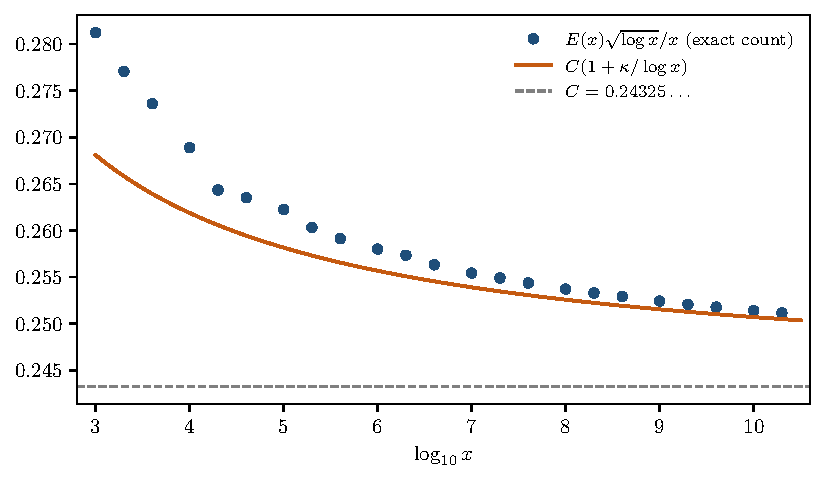
\includegraphics[width=0.75\textwidth]{figures/fig3_exceptions.pdf}
\caption{$\E(x)\sqrt{\log x}/x$ for $10^3\le x\le2\cdot10^{10}$, $x=c\cdot10^k$ with $c\in\{1,2,4\}$, against the limit $C$ and the two-term curve $C(1+\kappa/\log x)$ of Theorem~\ref{thm:exc}.}
\label{fig:exc}
\end{figure}

\begin{figure}[htbp]
\centering
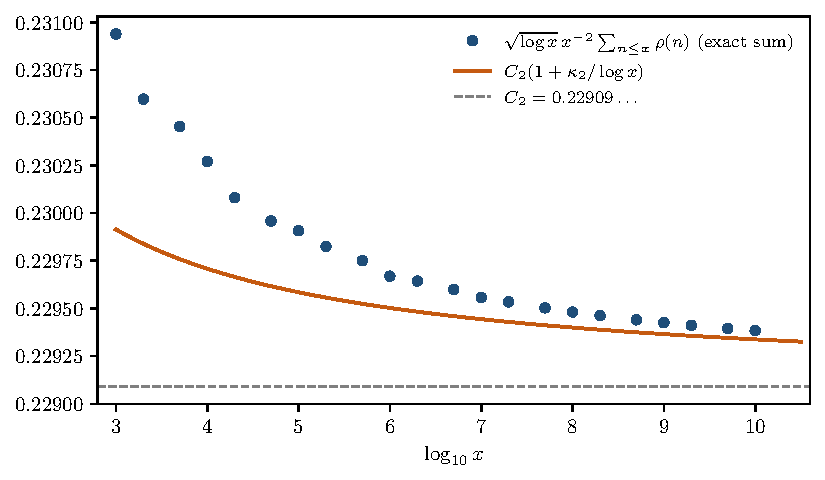
\includegraphics[width=0.75\textwidth]{figures/fig4_rho_sum.pdf}
\caption{$x^{-2}\sqrt{\log x}\sum_{n\le x}\rho(n)$ for $10^3\le x\le10^{10}$, $x=c\cdot10^k$ with $c\in\{1,2,5\}$, against the limit $C_2$ and the two-term curve $C_2(1+\kappa_2/\log x)$ of Theorem~\ref{thm:mean}.}
\label{fig:mean}
\end{figure}

%% ===================================================================
\section{Conclusions}\label{sec:conc}
%% ===================================================================

The ratio of surjective group homomorphisms to ring homomorphisms $\Z_m\to\Z_n$ is $2^{\epsilon(n)}|U_n^2|$, with $\epsilon(n)$ determined by the $2$-part of $n$, and it is an integer exactly off the set $\E$ of $n\equiv2\pmod4$ whose odd part has only prime factors $\equiv3\pmod4$. For odd $n$ the ring homomorphisms are in canonical bijection with the subfields of $\Q(\zeta_n)$ of degree at most $2$, and $\rho(n)$ is the degree of $\Q(\zeta_n)$ over its maximal multiquadratic subfield. The set $\E$ has $Cx(\log x)^{-1/2}(1+\kappa/\log x+O((\log x)^{-2}))$ elements up to $x$, and the partial sums of $\rho$ are $C_2x^2(\log x)^{-1/2}(1+\kappa_2/\log x+O((\log x)^{-2}))$, with all four constants explicit and confirmed by exact computation to $2\cdot10^{10}$ and $10^{10}$ respectively. The same method gives further terms of both expansions, at the cost of higher derivatives of $L(s,\chi_{-4})$ and of the Euler products at $s=1$.

\section*{Author contributions}

[To be completed by the authors.]

\section*{Use of AI tools declaration}

[To be completed by the authors.]

\section*{Acknowledgments}

The authors thank Prof.\ Jaikumar Radhakrishnan (ICTS-TIFR, Bengaluru) for helpful comments.

\section*{Funding}

The authors did not receive any financial support for the research, authorship, or publication of this article.

\section*{Conflict of interest}

The authors declare no conflicts of interest.

\section*{Data availability}

The C and Python programs and the exact counts behind Tables~\ref{tab:exc} and~\ref{tab:mean} are available at \url{https://github.com/creelie/quadratic-residue}.

\begin{thebibliography}{9}
\setlength{\itemsep}{1pt}
\small

\bibitem{GVB}
J. A. Gallian, J. Van Buskirk, The number of homomorphisms from $\Z_m$ into $\Z_n$, \textit{Amer. Math. Mon.}, \textbf{91} (1984), 196--197. \url{https://doi.org/10.1080/00029890.1984.11971375}

\bibitem{Moree}
P. Moree, Chebyshev's bias for composite numbers with restricted prime divisors, \textit{Math. Comp.}, \textbf{73} (2004), 425--449. \url{https://doi.org/10.1090/S0025-5718-03-01536-9}

\bibitem{JZ}
G. A. Jones, A. K. Zvonkin, A number-theoretic problem concerning pseudo-real Riemann surfaces, \textit{Integers}, \textbf{25} (2025), A75. \url{https://doi.org/10.5281/zenodo.16881820}

\bibitem{FS}
S. Finch, P. Sebah, Squares and cubes modulo $n$, \textit{arXiv:math/0604465v3}, 2016. \url{https://doi.org/10.48550/arXiv.math/0604465}

\bibitem{Ten}
G. Tenenbaum, \textit{Introduction to analytic and probabilistic number theory}, 3 Eds., Providence: American Mathematical Society, 2015. \url{https://doi.org/10.1090/gsm/163}

\bibitem{IR}
K. Ireland, M. Rosen, \textit{A classical introduction to modern number theory}, 2 Eds., New York: Springer, 1990. \url{https://doi.org/10.1007/978-1-4757-2103-4}

\bibitem{Wash}
L. C. Washington, \textit{Introduction to cyclotomic fields}, 2 Eds., New York: Springer, 1997. \url{https://doi.org/10.1007/978-1-4612-1934-7}

\bibitem{MV}
H. L. Montgomery, R. C. Vaughan, \textit{Multiplicative number theory I: Classical theory}, Cambridge: Cambridge University Press, 2006. \url{https://doi.org/10.1017/CBO9780511618314}

\end{thebibliography}

\end{document}
